%
%===============>>  Сорокин Модуль 6 <<=============
%=
\setmodule{6}

%BEGIN_FOLD % ====>>_____ Занятие 1 _____<<====
\begin{class}[number=1]
	\begin{definit}
		Сумма внутренних углов в треугольнике равна \( 180\degree \).
	\end{definit}
	\begin{definit}
		\textbf{Внешний угол} --- угол между стороной треугольника и продолжением другой стороны. Внешний угол является смежным с одним из внутренних.
	\end{definit}
	\begin{listofex}
		\item В треугольнике \( ABC \) два угла равны \( 50\) и \( 70 \) градусов. Найдите третий угол.
		\item Один угол треугольника равен \( 26\degree \), а второй в три раза больше. Найдите третий угол.
		\item Один внутренний угол треугольника в два, а второй в три раза больше третьего, найдите все углы треугольника.
		\item Один внешний угол равен \( 40\degree \), а второй --- \( 100\degree \). Чему равны внутренние углы треугольника?
		\item Угол треугольника равен \( 30\degree \), второй угол в \( 3 \) раза больше первого. Чему равны внешние углы при каждой вершине? Чему равна сумма внешних углов?
		\item В прямоугольном треугольнике один угол равен \( 40 \) градусов. Найдите сумму наибольшего и наименьшего угла.
		\item В прямоугольном треугольнике один острый угол на \( 17 \) градусов больше другого. Найдите углы треугольника.
		\item В прямоугольном треугольнике два острых угла равны. Какая у них градусная мера?
		
	\end{listofex}
	\begin{definit}
		Если секущая пересекает две параллельные прямые, то:
		\begin{tasks}(1)
			\task внутренние накрест лежащие углы равны: \( \angle 4 \) и \( \angle5 \), \( \angle 3 \) и \( \angle 6\);
			\task сумма внутренних односторонних углов равна  \(180\degree\): \( \angle 3 \) и \( \angle 5 \), \( \angle 4 \) и \( \angle 6 \);
			\task соответственные углы равны: \( \angle 1 \) и \( \angle 5 \), \( \angle 2 \) и \( \angle 6 \), \( \angle 3 \) и \( \angle 7 \), \( \angle 4 \) и \( \angle 8 \);
			\task внешние накрест лежащие углы равны: \( \angle 2 \) и \( \angle 7 \), \( \angle 1 \) и \( \angle 8 \);
			\task сумма внешних односторонних углов равна  \(180\degree\): \( \angle 1 \) и \( \angle 7 \), \( \angle 2 \) и \( \angle 8 \).
		\end{tasks}
	\begin{minipage}[c]{0.9\linewidth}
		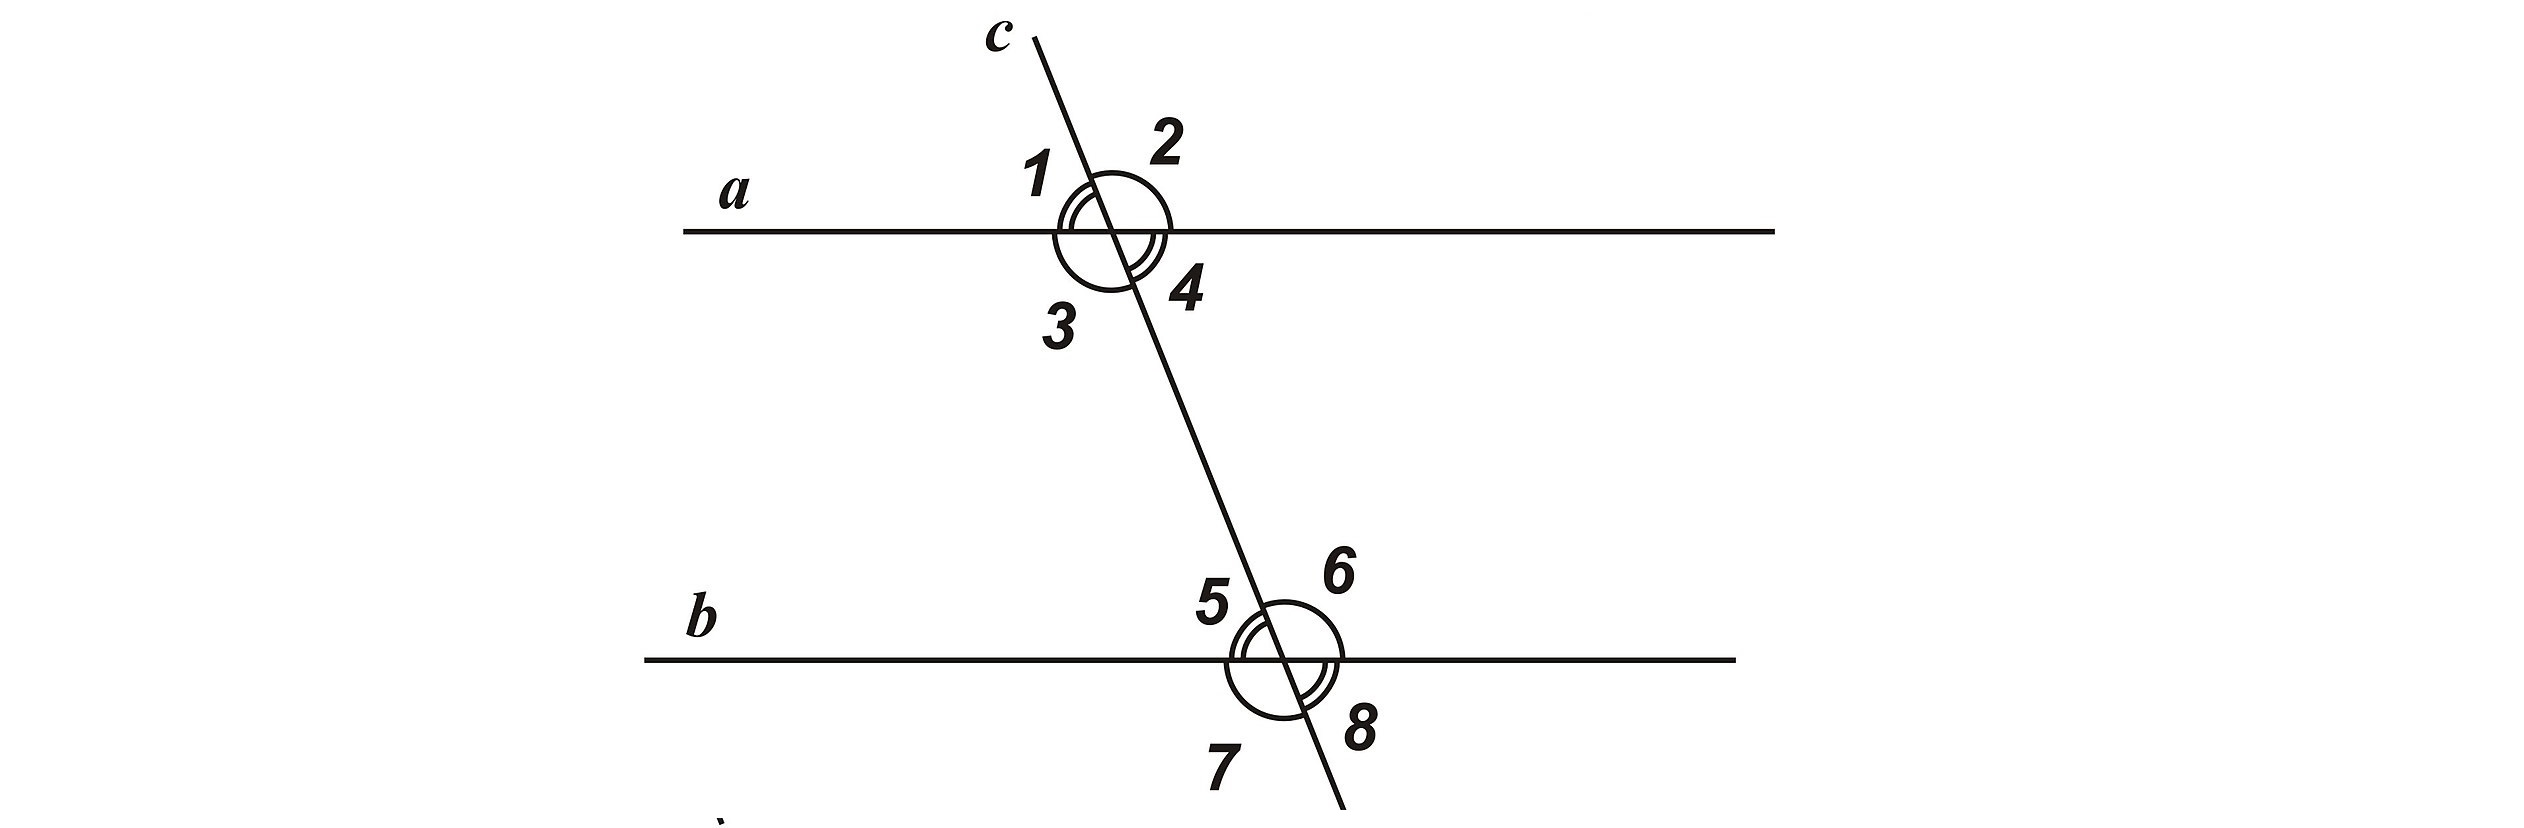
\includegraphics[align=t, width=\linewidth]{../\picpath/sorokinM6L1-1}
	\end{minipage}
	\end{definit}
	\begin{listofex}[resume]
		\item Сумма накрест лежащих углов при пересечении двух параллельных прямых секущей равна \(210 \degree \). Найдите эти углы.
		\item Найдите все углы, образованные при пересечении параллельных прямых \(a\) и \(b\) с секущей \(c\), если один из углов равен \( 150 \degree \).
		\item Через вершину \(C\) треугольника \(ABC\) проведена прямая, параллельная биссектрисе \(BD\) угла \(ABC\). Эта прямая пересекает прямую \(AB\) в точке \(K\). Найдите углы треугольника \(BKC\), если \(\angle ABC = 130 \degree\).
		\item Через вершину \(B\) треугольника \(ABC\) проведена прямая, параллельная прямой \(AC\). Образовавшиеся при этом три угла с вершиной B относятся как \(3 : 10 : 5\). Найдите углы треугольника \(ABC\).
		\item Через середину \(M\) отрезка с концами на двух параллельных прямых проведена прямая, пересекающая эти прямые в точках \(A\) и \(B\). Докажите, что \(M\) также середина \(AB\).
		\item Внешние углы треугольника \(ABC\) при вершинах \(A\) и \(C\) равны \(115\degree\) и \(140\degree \). Прямая, параллельная прямой \(AC\), пересекает стороны \(AB\) и \(AC\) в точках \(M\) и \(N\). Найдите углы треугольника \(BMN\).
		\item Через точку \(M\), лежащую внутри угла с вершиной \(A\), проведены прямые, параллельные сторонам угла и пересекающие эти стороны в точках \(B\) и \(C\). Известно, что \(\angle ACB = 50\degree\), а угол, смежный с углом \(ACM\), равен \(40\degree\). Найдите углы треугольников \(BCM\) и \(ABC\).
		\item Прямая пересекает боковую сторону \(AC\), основание \(BC\) и продолжение боковой стороны \(AB\) равнобедренного треугольника \(ABC\) за точку \(B\) в точках \(K, L\) и \(M\) соответственно. При этом треугольники \(CKL\) и \(BML\) получаются также равнобедренными. Найдите их углы.
		%\item Отрезки \(AB\) и \(CD\) пересекаются в точке \(O\) и делятся этой
	\end{listofex}
\end{class}
%END_FOLD

%BEGIN_FOLD % ====>>_ Домашняя работа 1 _<<====
\begin{homework}[number=1]
	\begin{listofex}
		\item В прямоугольном треугольнике один острый угол на \( 25 \) градусов больше другого. Найдите острые углы треугольника.
		\item Угол треугольника равен \( 36\degree \), второй угол в \( 2 \) раза меньше первого. Чему равны внешние углы при каждой вершине? Чему равна сумма внешних углов?
		\item Сумма соответственных углов при пересечении двух параллельных прямых секущей равна \(190\degree \). Найдите эти углы.
		\item Накрест лежащие углы, образованные при пересечении двух параллельных прямых третьей, в сумме составляют \(80\) градусов. Найдите все углы, образовавшиеся при пересечении параллельных прямых секущей.
		\item Найдите все углы, образованные при пересечении параллельных прямых \(a\) и \(b\) с секущей \(c\), если один из углов равен \( 115 \degree \).
		%\item \(AD\) --- биссектриса треугольника \(ABC\). Точка \(M\) лежит на стороне \(AB\), причем \(AM = MD\). Докажите, что \(MD \parallel AC\).
		%\item Точки \(A\) и \(D\) лежат на одной из двух параллельных прямых, точки \(B\) и \(C\) --- на другой, причем прямые \(AB\) и \(CD\) также параллельны. Докажите, что \(AB = CD\) и \(AD = BC\).
		%\item Треугольник \(ABC\) --- равнобедренный \((AB = BC)\). Отрезок \(AM\) делит его на два равнобедренных треугольника с основаниями \(AB\) и \(MC\). Найдите угол \(B\).
		\item Углы треугольника относятся как \(2 : 3 : 4\). Найдите отношение внешних углов треугольника.
		%\item Равные отрезки \(AB\) и \(CD\) пересекаются в точке \(O\) и делятся ею в отношении \(AO : OB = CO : OD = 1 : 2\). Прямые \(AD\) и \(BC\) пересекаются в точке \(M\). Докажите, что треугольник \(DMB\) равнобедренный.
		\item Точки \(A\) и \(D\) лежат на одной из двух параллельных прямых, точки \(B\) и \(C\) --- на другой, причем прямые \(AB\) и \(CD\) также параллельны. Докажите, что противоположные углы четырехугольника \(ABCD\) равны между собой.
	\end{listofex}
\end{homework}
%END_FOLD

%BEGIN_FOLD % ====>>_____ Занятие 2 _____<<====
\begin{class}[number=2]
	\begin{listofex}
		\item Занятие 2
	\end{listofex}
\end{class}
%END_FOLD

%BEGIN_FOLD % ====>>_ Домашняя работа 2 _<<====
\begin{homework}[number=2]
	\begin{listofex}
		\item Домашняя работа
	\end{listofex}
\end{homework}
%END_FOLD

%BEGIN_FOLD % ====>>_____ Занятие 3 _____<<====
\begin{class}[number=3]
	\begin{listofex}
		\item Занятие 3
	\end{listofex}
\end{class}
%END_FOLD

%BEGIN_FOLD % ====>>_ Домашняя работа 3 _<<====
\begin{homework}[number=3]
	\begin{listofex}
		\item Домашняя работа
	\end{listofex}
\end{homework}
%END_FOLD

%BEGIN_FOLD % ====>>_____ Занятие 4 _____<<====
\begin{class}[number=4]
	\begin{listofex}
		\item Пусто
	\end{listofex}
\end{class}
%END_FOLD


%BEGIN_FOLD % ====>>_ Проверочная работа _<<====
\begin{exam}
	\begin{listofex}
		\item Проверочная
	\end{listofex}
\end{exam}
%END_FOLD